% Requires \usepackage{graphicx}. Paths assume the PDFs are next to the paper.
% These are stand-alone insertion snippets; the main article is not modified.
\begin{figure*}[t]
  \centering
  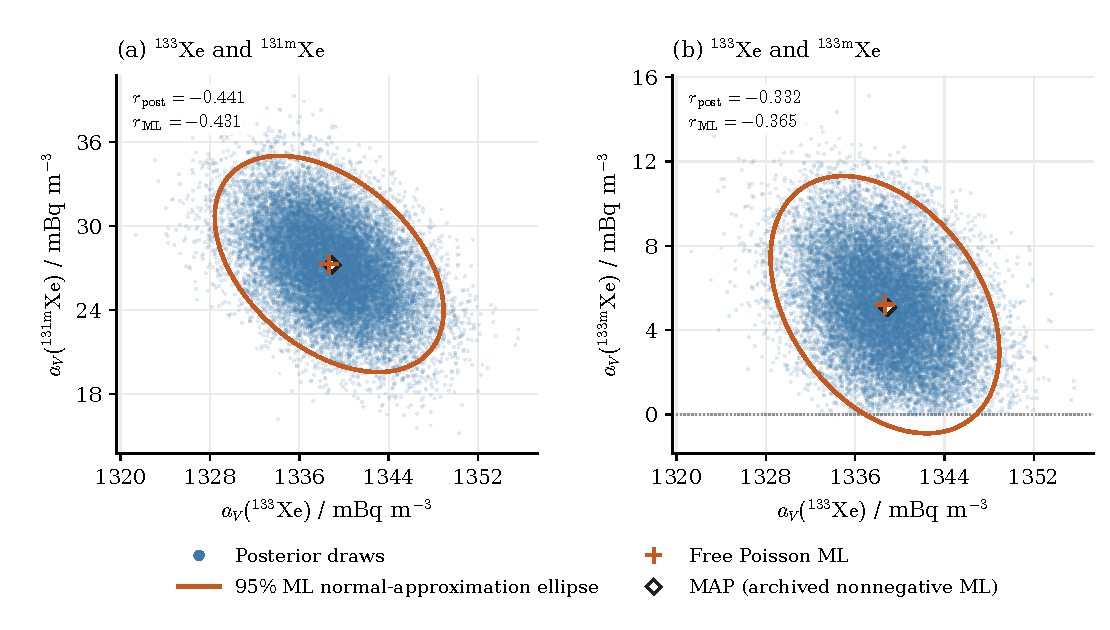
\includegraphics[width=\textwidth]{bayesian_joint_concentrations.pdf}
  \caption{Joint posterior distributions of the fresh-sample concentrations
  for the original August measurement: (a) $^{133}$Xe and $^{131\mathrm{m}}$Xe;
  (b) $^{133}$Xe and $^{133\mathrm{m}}$Xe. The joint Poisson model includes
  SAMPLE, GASBK, and DETBK, with all 17 physical parameters inferred jointly
  under a constant prior on the nonnegative orthant. Calibrations are fixed.
  The ellipses are the original free Poisson maximum-likelihood (ML) normal
  approximations using the full propagated statistical covariance and
  $\chi^2_{2,0.95}=5.99146$; they are not posterior credible regions.
  Crosses mark the free ML estimates, and diamonds mark the archived
  nonnegative ML estimates, which serve as the physical-space MAP reference.}
  \label{fig:xemat-bayesian-joint-original}
\end{figure*}

\begin{figure*}[t]
  \centering
  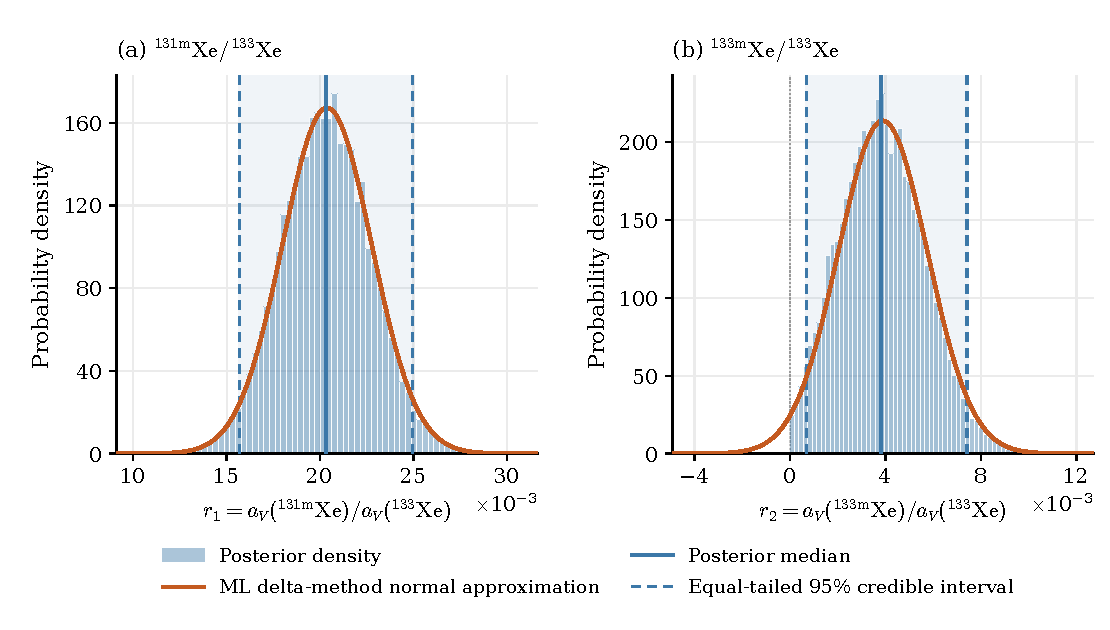
\includegraphics[width=\textwidth]{bayesian_ratios.pdf}
  \caption{Posterior distributions of (a)
  $r_1=a_V(^{131\mathrm{m}}\mathrm{Xe})/a_V(^{133}\mathrm{Xe})$ and (b)
  $r_2=a_V(^{133\mathrm{m}}\mathrm{Xe})/a_V(^{133}\mathrm{Xe})$ for the
  original August measurement. Ratios are calculated within each joint
  posterior draw, preserving parameter correlations. Solid blue lines mark
  posterior medians; dashed blue lines delimit equal-tailed 95\% credible
  intervals. Orange curves show the normal delta-method approximations
  about the original free Poisson ML estimates, including the covariance
  cross terms. Their negative tails are retained without truncation or
  renormalization. All comparisons condition on the original model and
  fixed calibrations.}
  \label{fig:xemat-bayesian-ratios-original}
\end{figure*}
